\documentclass[border=8pt]{standalone}
\usepackage{amsmath,amssymb,bm}
\usepackage{xcolor}
\usepackage{tikz}
\definecolor{P}{HTML}{49B7B1}
\definecolor{ink}{HTML}{1B1B2F}
\colorlet{band}{P!7!white}
\colorlet{lcol}{P!18!white}
\colorlet{rule}{P!45!white}
\colorlet{Pd}{P!80!white}
\begin{document}
\large
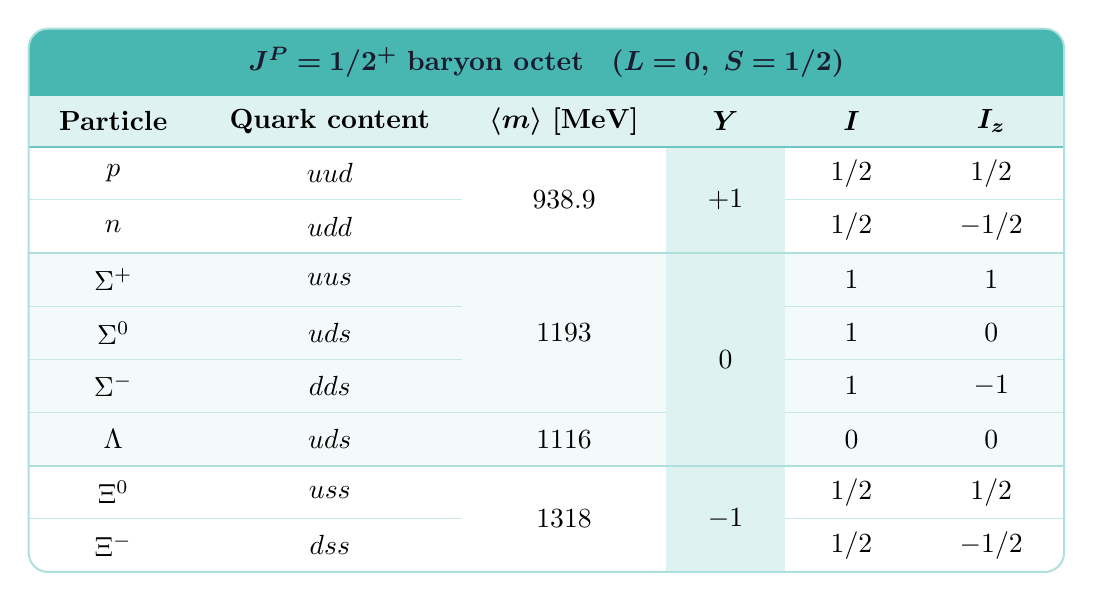
\begin{tikzpicture}
  \begin{scope}
    \clip[rounded corners=7pt] (0,0) rectangle (13.150,-6.900);
    \fill[P] (0,0) rectangle (13.150,-0.850);
    \fill[lcol] (0,-0.850) rectangle (13.150,-1.500);
    \fill[band] (0,-2.850) rectangle (13.150,-5.550);
    \fill[lcol] (8.100,-1.500) rectangle (9.600,-6.900);
  \end{scope}
  \draw[rule!70,line width=.35pt] (0.000,-2.175) -- (5.500,-2.175) (9.600,-2.175) -- (13.150,-2.175);
  \draw[rule,line width=.7pt] (0,-2.850) -- (13.150,-2.850);
  \draw[rule!70,line width=.35pt] (0.000,-3.525) -- (5.500,-3.525) (9.600,-3.525) -- (13.150,-3.525);
  \draw[rule!70,line width=.35pt] (0.000,-4.200) -- (5.500,-4.200) (9.600,-4.200) -- (13.150,-4.200);
  \draw[rule!70,line width=.35pt] (0.000,-4.875) -- (8.100,-4.875) (9.600,-4.875) -- (13.150,-4.875);
  \draw[rule,line width=.7pt] (0,-5.550) -- (13.150,-5.550);
  \draw[rule!70,line width=.35pt] (0.000,-6.225) -- (5.500,-6.225) (9.600,-6.225) -- (13.150,-6.225);
  \draw[Pd,line width=.7pt] (0,-1.500) -- (13.150,-1.500);
  \draw[rule,line width=.7pt,rounded corners=7pt] (0,0) rectangle (13.150,-6.900);
  \node[text=ink,align=center] at (6.575,-0.425) {$\bm{J^{P}=1/2^{+}}\ \textbf{baryon octet}\quad \bm{(L=0,\ S=1/2)}$};
  \node at (1.075,-1.175) {\textbf{Particle}};
  \node at (3.825,-1.175) {\textbf{Quark content}};
  \node at (6.800,-1.175) {$\bm{\langle m\rangle}$ \textbf{[MeV]}};
  \node at (8.850,-1.175) {$\bm{Y}$};
  \node at (10.450,-1.175) {$\bm{I}$};
  \node at (12.225,-1.175) {$\bm{I_z}$};
  \node at (1.075,-1.837) {$p$};
  \node at (3.825,-1.837) {$uud$};
  \node at (12.225,-1.837) {$1/2$};
  \node at (10.450,-1.837) {$1/2$};
  \node at (1.075,-2.513) {$n$};
  \node at (3.825,-2.513) {$udd$};
  \node at (12.225,-2.513) {$-1/2$};
  \node at (10.450,-2.513) {$1/2$};
  \node at (1.075,-3.188) {$\Sigma^{+}$};
  \node at (3.825,-3.188) {$uus$};
  \node at (12.225,-3.188) {$1$};
  \node at (10.450,-3.188) {$1$};
  \node at (1.075,-3.863) {$\Sigma^{0}$};
  \node at (3.825,-3.863) {$uds$};
  \node at (12.225,-3.863) {$0$};
  \node at (10.450,-3.863) {$1$};
  \node at (1.075,-4.537) {$\Sigma^{-}$};
  \node at (3.825,-4.537) {$dds$};
  \node at (12.225,-4.537) {$-1$};
  \node at (10.450,-4.537) {$1$};
  \node at (1.075,-5.213) {$\Lambda$};
  \node at (3.825,-5.213) {$uds$};
  \node at (12.225,-5.213) {$0$};
  \node at (10.450,-5.213) {$0$};
  \node at (1.075,-5.888) {$\Xi^{0}$};
  \node at (3.825,-5.888) {$uss$};
  \node at (12.225,-5.888) {$1/2$};
  \node at (10.450,-5.888) {$1/2$};
  \node at (1.075,-6.562) {$\Xi^{-}$};
  \node at (3.825,-6.562) {$dss$};
  \node at (12.225,-6.562) {$-1/2$};
  \node at (10.450,-6.562) {$1/2$};
  \node at (8.850,-2.175) {$+1$};
  \node at (8.850,-4.200) {$0$};
  \node at (8.850,-6.225) {$-1$};
  \node at (6.800,-2.175) {$938.9$};
  \node at (6.800,-3.863) {$1193$};
  \node at (6.800,-5.213) {$1116$};
  \node at (6.800,-6.225) {$1318$};
\end{tikzpicture}
\end{document}
